\documentclass[10pt]{article}
\usepackage[utf8]{inputenc}
\usepackage[T1]{fontenc}
\usepackage{amsmath}
\usepackage{amsfonts}
\usepackage{amssymb}
\usepackage[version=4]{mhchem}
\usepackage{stmaryrd}
\usepackage{graphicx}
\usepackage[export]{adjustbox}
\usepackage{caption}

\DeclareUnicodeCharacter{00D7}{\ifmmode\times\else{$\times$}\fi}

\begin{document}

\section*{Theory 9: 'Second eclipse'}
For each of two eclipsing binaries A and B, the primary eclipses were observed with very high cadence as depicted below:

\begin{figure}[h]
\begin{center}
  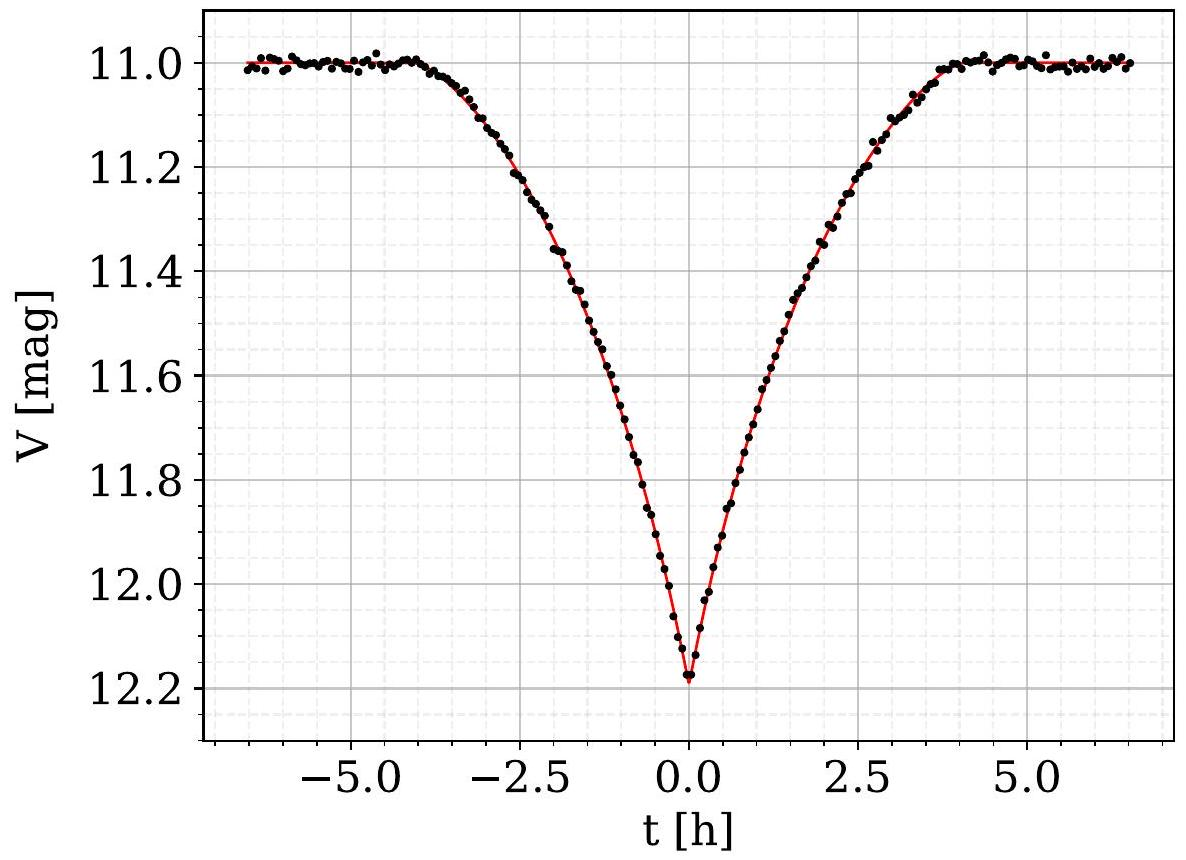
\includegraphics[width=\textwidth]{2025_09_11_9b0a1b7404262e10b3c8g-07}
\captionsetup{labelformat=empty}
\caption{Figure 1: Observed lightcurve for system A.}
\end{center}
\end{figure}

\begin{figure}[h]
\begin{center}
  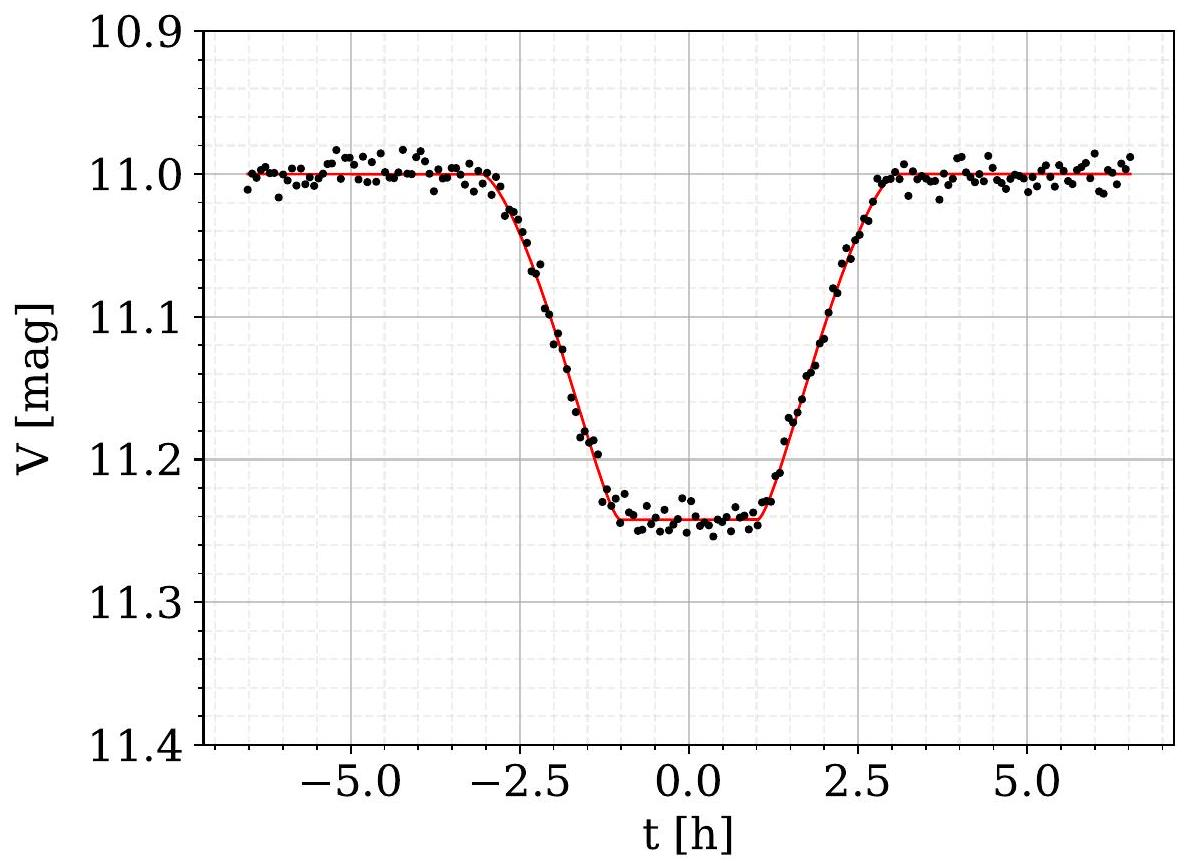
\includegraphics[width=\textwidth]{2025_09_11_9b0a1b7404262e10b3c8g-07(1)}
\captionsetup{labelformat=empty}
\caption{Figure 2: Observed lightcurve for system B.}
\end{center}
\end{figure}

In the figures, $t$ is the time in hours relative to the moment of minimum and $V$ is the brightness in the $V$ (visible) band in magnitudes. The points are the measurements and the line is the fitted model of the shape of the eclipse.

You can assume that in both cases the eclipses are central ( $i=90^{\circ}$ ) and last for a very small fraction of the orbital period, limb darkening is negligible, and the orbits have low eccentricity.

On the Answer Sheet, draw the predicted shape of the light curve for each of the secondary eclipses. Write down the equations and calculations leading to your predictions.\\
(20 points)

\section*{Answer Sheet}
\begin{figure}[h]
\begin{center}
  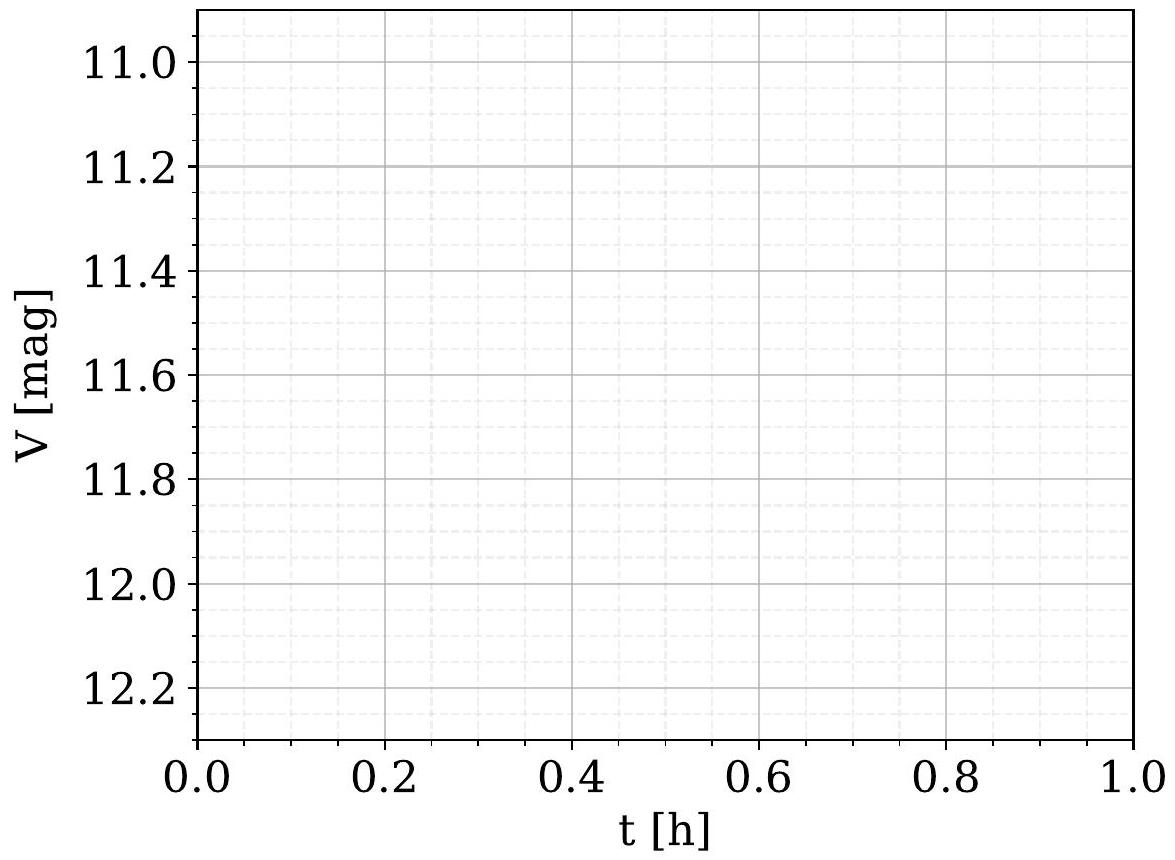
\includegraphics[width=\textwidth]{2025_09_11_9b0a1b7404262e10b3c8g-09}
\captionsetup{labelformat=empty}
\caption{Figure 3: Predicted lightcurve for the second eclipse for system A.}
\end{center}
\end{figure}

\begin{figure}[h]
\begin{center}
  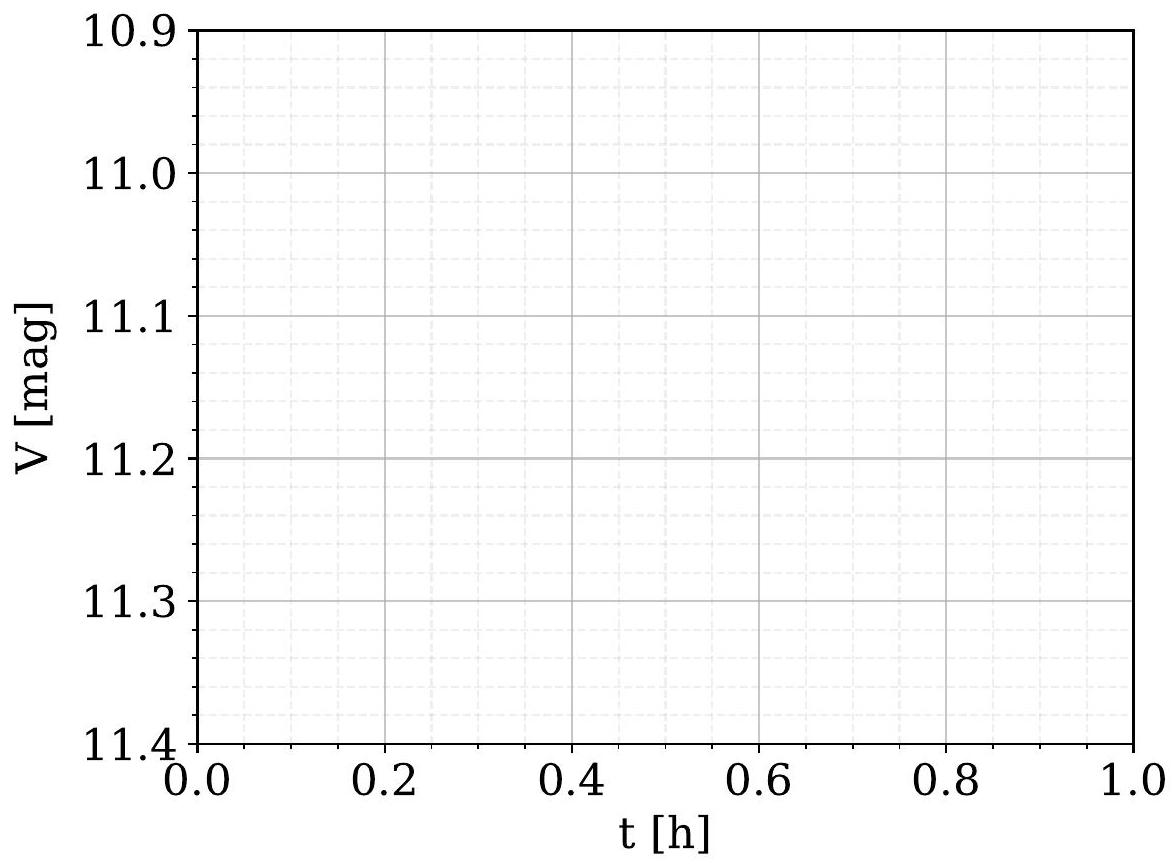
\includegraphics[width=\textwidth]{2025_09_11_9b0a1b7404262e10b3c8g-09(1)}
\captionsetup{labelformat=empty}
\caption{Figure 4: Predicted lightcurve for the second eclipse for system B.}
\end{center}
\end{figure}

\end{document}